\documentclass[11pt]{article}
\usepackage[english]{babel}
\usepackage{geometry}
\usepackage{amsmath}
\usepackage{amsthm}
\usepackage[draft]{graphicx}
\usepackage{float}
\usepackage[utf8]{inputenc}

\graphicspath{{../src/plts/}}

%%%%%%%% MARGIN
\geometry{verbose, letterpaper, tmargin=3cm,
  bmargin=3cm,lmargin=2.5cm,rmargin=2.5cm}

%%%%%%%% PARAGRAPH SETTINGS
% https://tex.stackexchange.com/questions/27802/set-noindent-for-entire-file
\setlength\parindent{0pt}

% https://tex.stackexchange.com/questions/49188/how-to-insert-vertical-space-between-paragraphs
\setlength{\parskip}{5pt}

%%%%%%%% SUB-FIGURE PACKAGE
\usepackage{subcaption}

%%%%%%%% HYPERREF PACKAGE
\usepackage{hyperref}
\hypersetup{linkcolor=blue}
\hypersetup{citecolor=blue}
\hypersetup{urlcolor=blue}
\hypersetup{colorlinks=true}

%%%%%%%% DEFINITION AND THEOREM DEFINITIONS
\theoremstyle{definition}
\newtheorem{definition}{Definition}[section]

\theoremstyle{remark}
\newtheorem{remark}{Remark}

\theoremstyle{remark}
\newtheorem{question}{Question}

\newtheorem{theorem}{Theorem}[section]

%%%%%%%% MULTI-COLUMNS PACKAGE
\usepackage{multicol}

%%%%%%%% BIB-LATEX STUFF
\usepackage[style=numeric,
            bibstyle=numeric,
            citestyle=numeric,
            hyperref=true,
            backend=biber]{biblatex}
\addbibresource{ref.bib}

%%%%%%%% PERSONAL COMMANDS
\usepackage{amssymb}

%%%% Important sets
\renewcommand{\O}{\mathbb{O}}
\newcommand{\N}{\mathbb{N}}
\newcommand{\Z}{{\mathbb{Z}}}
\newcommand{\Q}{{\mathbb{Q}}}
\newcommand{\R}{{\mathbb{R}}}

%%%% Lambda Calculus Symbols
\newcommand{\dneq}{\,\, \# \,\,}
\renewcommand{\S}{\pmb{\mathrm{S}}}
\newcommand{\I}{\pmb{\mathrm{I}}}
\newcommand{\K}{\pmb{\mathrm{K}}}
\newcommand{\ch}[1]{\ulcorner #1 \urcorner}

%%%% Ordinal Lambda Calculus Symbols
\newcommand{\ordAlph}{\Sigma_{\text{Ord}}}
\newcommand{\termOrd}{\text{Term}_\text{Ord}}
\newcommand{\fl}{\mathrm{fl}}
\newcommand{\sk}{\mathrm{sk}}

%%%% Superscript to the left
% https://latex.org/forum/viewtopic.php?t=455
\usepackage{tensor}
\newcommand{\app}[3]{\tensor*[^{#1}]{\left(#2, #3\right)}{}}

%%%% Make optional parameter
% https://tex.stackexchange.com/questions/217757/special-behavior-if-optional-argument-is-not-passed
\usepackage{xparse}

%%%% Statistics
\NewDocumentCommand{\E}{o m}{
  \IfNoValueTF{#1}
  {\mathbb{E}\left[#2\right]}
  {\mathbb{E}^{#1}\left[ #2\right]}
}
\NewDocumentCommand{\V}{o m}{
  \IfNoValueTF{#1}
  {\mathrm{Var}\left[#2\right]}
  {\mathrm{Var}^{#1}\left[ #2\right]}
}
\RenewDocumentCommand{\P}{o m}{
  \IfNoValueTF{#1}
  {\mathrm{P}\left(#2\right)}
  {\mathrm{P}^{#1}\left( #2\right)}
}

%%%% Lambda Calculus
\NewDocumentCommand{\cx}{o}{
  \IfNoValueTF{#1}
  {\left[\quad\right]}
  {\left[\, #1 \,\right]}
}

%%%%%%%% LOGIC TREES
\usepackage{prftree}

%%%%%%%% SPLIT EQUATIONS
% https://tex.stackexchange.com/questions/51682/is-it-possible-to-pagebreak-aligned-equations
\allowdisplaybreaks

%%%%%%%% TO USE SHORT COMMANDS FOR VECTOR LINES
\usepackage{esvect}

%%%%%%%% REFERENCES LAST PAGE
% https://tex.stackexchange.com/questions/320683/can-i-force-the-references-to-be-the-last-thing/320685
\usepackage{placeins}

%%%%%%%% CODE RENDERING %%%%%%% UN-COMMENT IF NECESSARY
% Compile with flag -shell-escape
% \usepackage{minted}

%%%%%%%% START DOCUMENT

\title{Stochastic Process Workshop}
\author{Juan Sebasti\'an C\'ardenas-Rodríguez \\
       David Plazas Escudero \\
       \scalebox{0.7}{Mathematical Engineering, Universidad EAFIT}}
\date{\today}


\begin{document}
\maketitle

The code for this workshop can be found in
\href{https://bit.ly/3ciL6Px}{source code}.

\section*{Prediction 1}
\begin{question}
  Suppose a variable can be modelled by a homogeneous linear
  differential equation with parameters $\Theta = \{\mu,
  \sigma\}$. Simulate a trajectory for a total of $N = 365$
  observations (days) and save the simulated trajectory (Series 1).
\end{question}

\begin{question}
  Construct three trajectories out the sample modifying the parameter
  $\mu$ for a total of $N = 365$. The trajectories must consider three
  scenarios optimistic, pessimistic and constant. Each trajectory must
  have as initial point the last point of Series 1.
\end{question}

\begin{question}
  Simulate multiple trajectories for Series 1 out of the historic
  information considering the three possible scenarios. Each
  trajectory will help to build a prediction band for each
  scenario. The bands can be constructed as combination of descriptive
  statistics obtained in the simulation of each trajectory
  longitudinally. Compare each confidence bands with data out the
  sample (scenarios). Determine the percentage of effectiveness of the
  bands. Conclude.
\end{question}

\begin{question}
  Make a sensitivity analysis of the simulated scenarios and their
  forecast respect to $\sigma$. Conclude.
\end{question}

The homogeneous linear stochastic differential equation (SDE) is given by

\begin{equation*}
  dX_t = \mu X_t dt + \sigma X_t dW_t
\end{equation*}

with $\{W_t\}_{t \ge 0}$ a Weiner process, $\mu \in \R$ and
$\sigma \in \R_+$.

The SDE was simulated using the Euler-Maruyama Method
\parencite{higham2001} in \texttt{Python}, with parameters $\mu = 0.003$,
$\sigma = 0.03$, $\Delta t = 1$, $t_f = 365$, $x_0 = 1$. It is important to
mention that the implemented algorithm for Euler-Maruyama runs in different
CPU cores simultaneously for speed execution and, additionally, the creation of
Weiner processes is run in parallel as well. This fact implies that, regardless
of a fixed seed for random number generation, the algorithm will return
different trajectories on each run, since each core is accessing the random
number generator simultaneously and not sequentially; therefore, the results
here presented are those of a single run.

The result of the simulation can be found in Figure \ref{fig:series1}. This
simulation will be known as Series 1. For the scenario simulation, we
modified the parameter $\mu$, in the
optimistic case, $\mu=0.007$ and, in the pessimistic case,
$\mu=-0.001$. The scenarios where simulated with the same $\Delta t$,
$\sigma$ and $t_0 = 365$, $t_f = 730$, $x_0=X_{t_0}$. The result of
the simulation of these scenarios can be found in \ref{fig:scenarios}.

\begin{figure}[H]
  \centering
  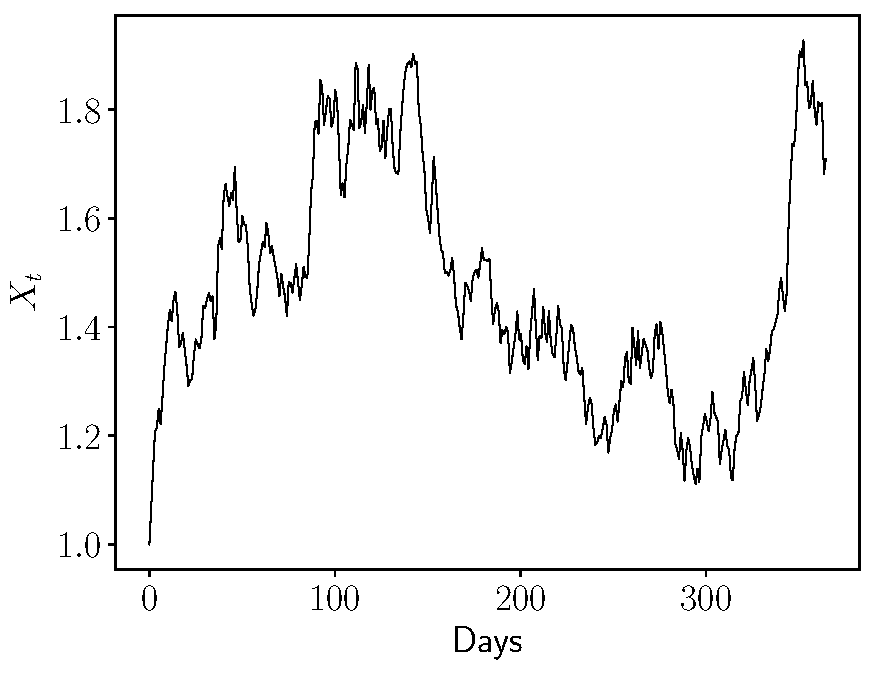
\includegraphics[scale=0.5]{series1.pdf}
  \caption{Series 1 simulation.}
  \label{fig:series1}
\end{figure}

\begin{figure}[H]
  \centering
  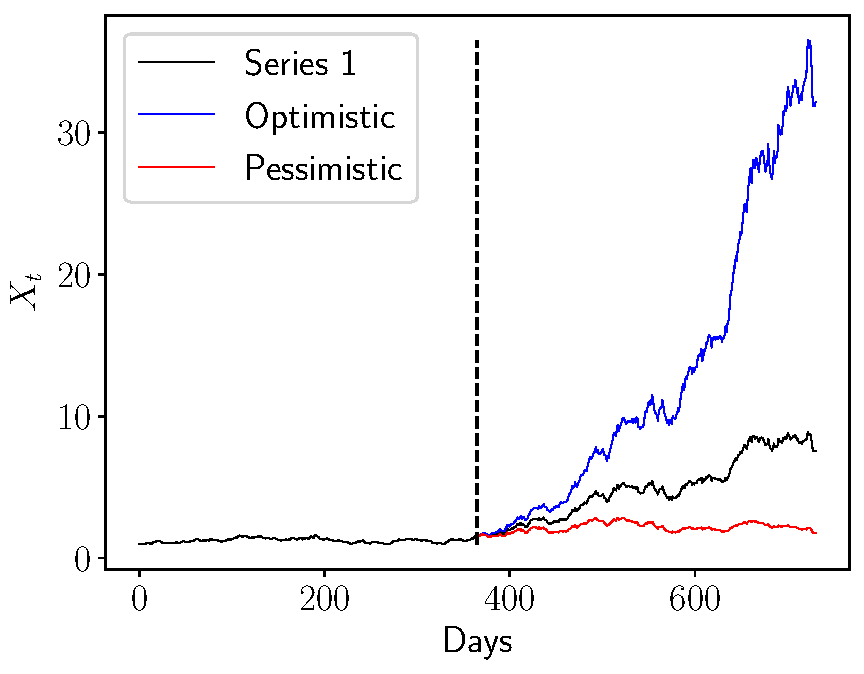
\includegraphics[scale=0.5]{pronostico-1-escenarios.pdf}
  \caption{Initial simulation with scenarios trajectories.}
  \label{fig:scenarios}
\end{figure}

Using the defined parameters, multiple trajectories for each scenario
were simulated. An example for 100 trajectories can be found in Figure
\ref{fig:trajectories1}. These figures show Series 1 along with the
trajectories of the respective scenario.

\begin{figure}[t]
  \centering
  \begin{subfigure}[b]{0.45\textwidth}
      \centering
      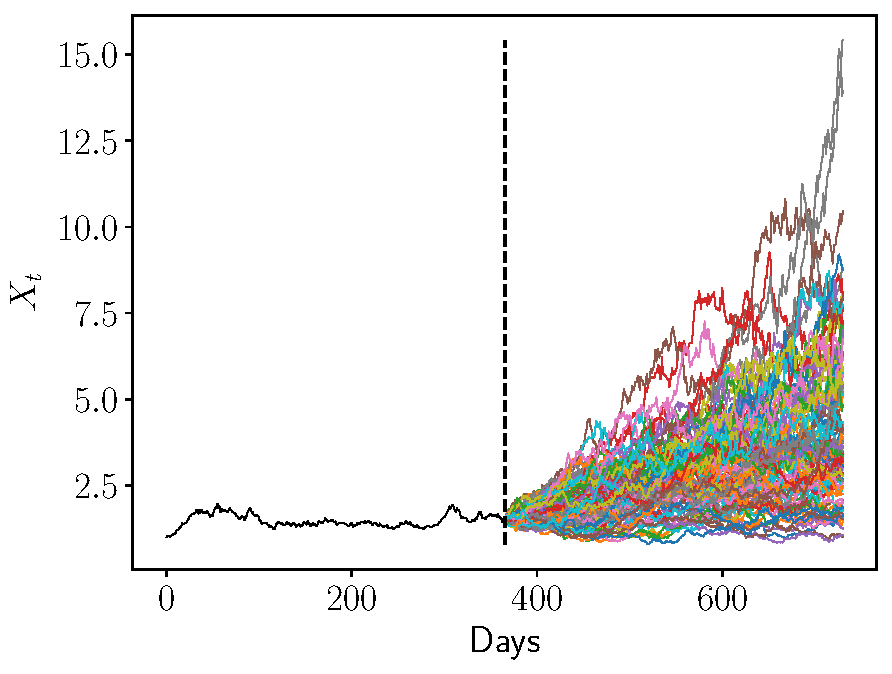
\includegraphics[scale=0.45]{pronostico-constante.pdf}
      \caption{Constant.}
  \end{subfigure}
  \begin{subfigure}[b]{0.45\textwidth}
      \centering
      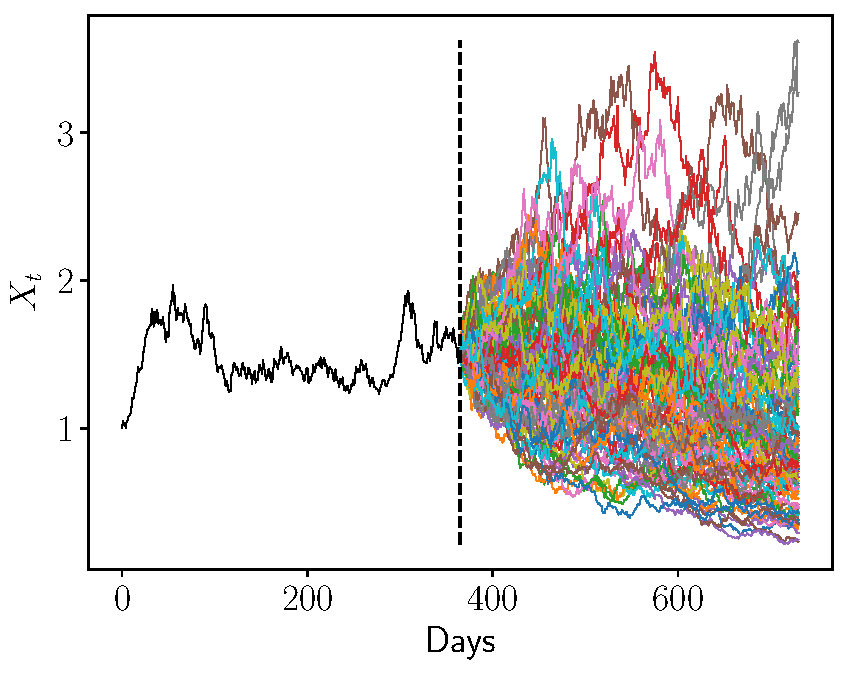
\includegraphics[scale=0.45]{pronostico-pesimista.pdf}
      \caption{Pessimistic.}
  \end{subfigure}
  \begin{subfigure}[b]{0.45\textwidth}
      \centering
      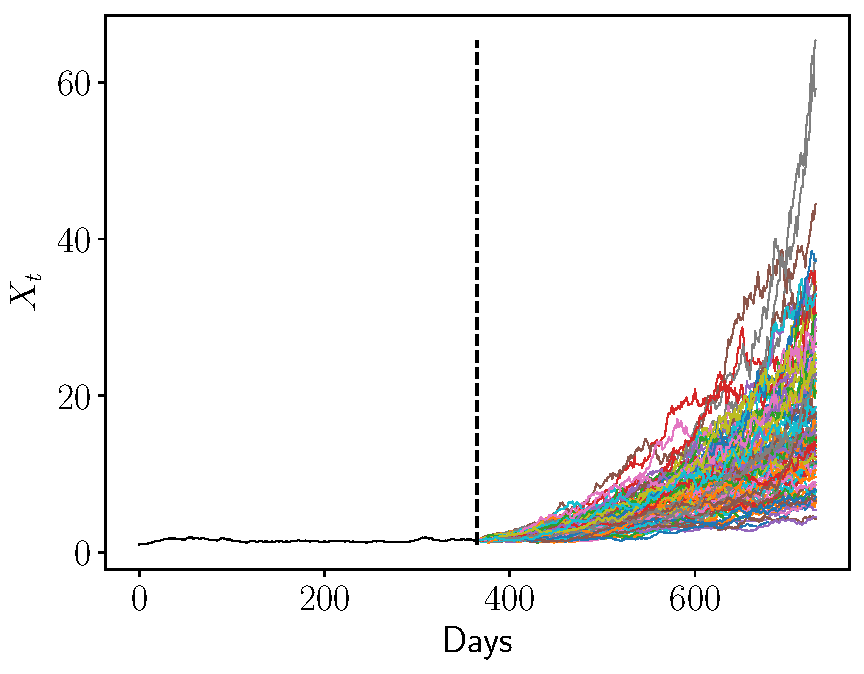
\includegraphics[scale=0.45]{pronostico-optimista.pdf}
      \caption{Optimistic.}
  \end{subfigure}
  \caption{Prediction trajectories for each scenario.}
  \label{fig:trajectories1}
\end{figure}

The procedure to obtain the prediction bands with a $1 - \alpha$
confidence is:
\begin{enumerate}
\item Simulate $n$ different trajectories with Euler-Maruyama, using
  $n$ different Weiner Processes.
\item For each $t \in (t_0, t_f]$ we fit a distribution
  $\hat{F}_t(\cdot)$ using the \texttt{scipy.stats} Python package.
\item For each $\hat{F}_t(\cdot)$ a goodness-of-fit test is done
  (Kolmogorov-Smirnov, Anderson-Darling, \dots).
\item For each $\hat{F}_t(\cdot)$ calculate the $\alpha / 2$ and
  $1 - \alpha/2$ quantiles. These yield a confidence interval at
  time $t$.
\end{enumerate}

Therefore, it is important to find the distribution for this
process. It is well known that the SDE is a Geometric Brownian Motion
and thus, it follows a lognormal distribution. Hence, the parameters
are fitted but the-goodness-of-fit test is not performed.

The prediction bands $\{B_t\}_{t \ge 0 }=\left(L_t, U_t\right)$
for each scenario are presented in Figure \ref{fig:pb1}, with
$\alpha=0.1$ and 1000 trajectories. It is important to notice that
Series 1 is no longer shown, only the prediction with the trajectories
of each scenario.

\begin{figure}[H]
  \centering
  \begin{subfigure}[b]{0.45\textwidth}
      \centering
      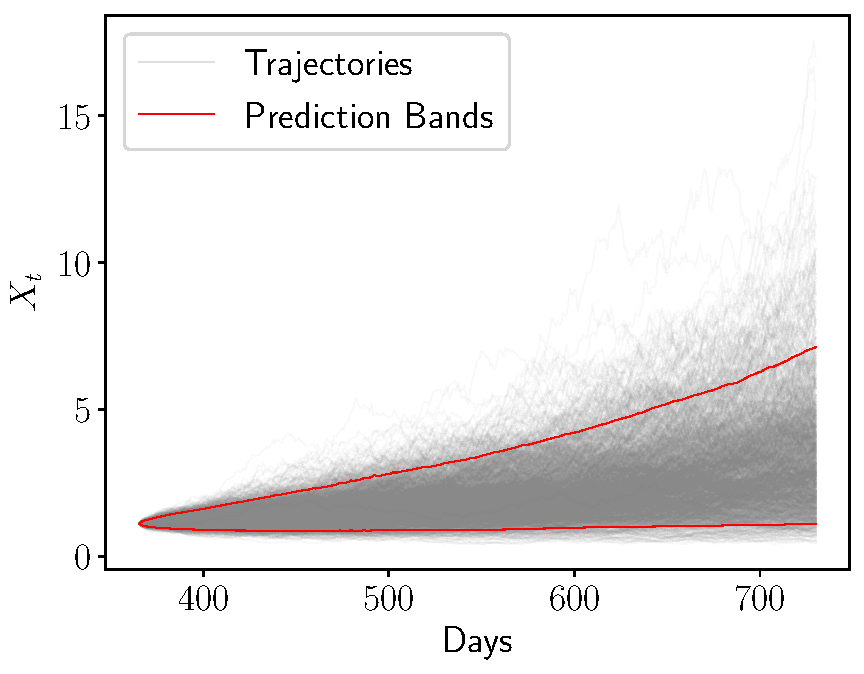
\includegraphics[scale=0.45]{bands_constant.pdf}
      \caption{Constant.}
  \end{subfigure}
  \begin{subfigure}[b]{0.45\textwidth}
      \centering
      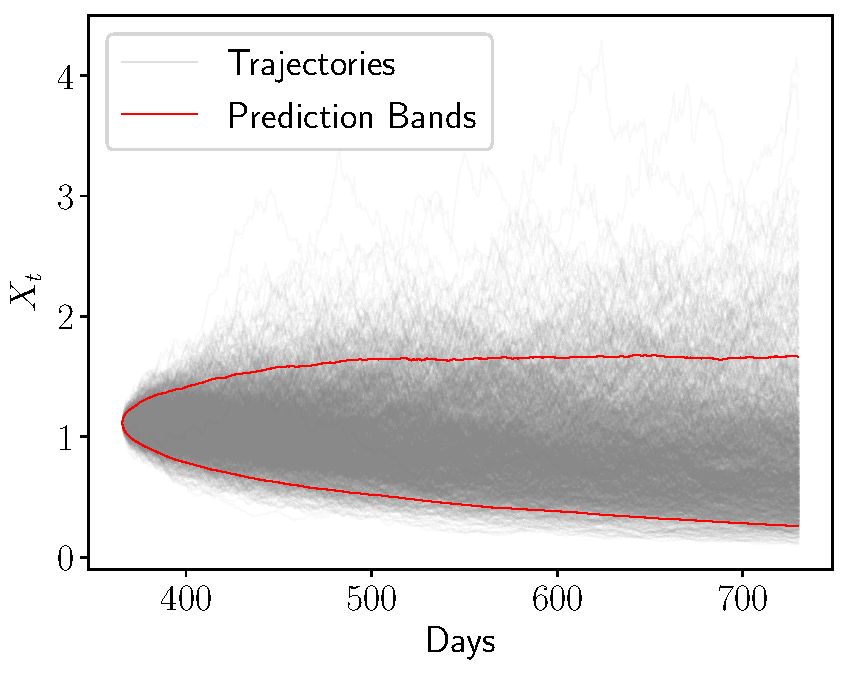
\includegraphics[scale=0.45]{bands_pessimistic.pdf}
      \caption{Pessimistic.}
  \end{subfigure}
  \begin{subfigure}[b]{0.45\textwidth}
      \centering
      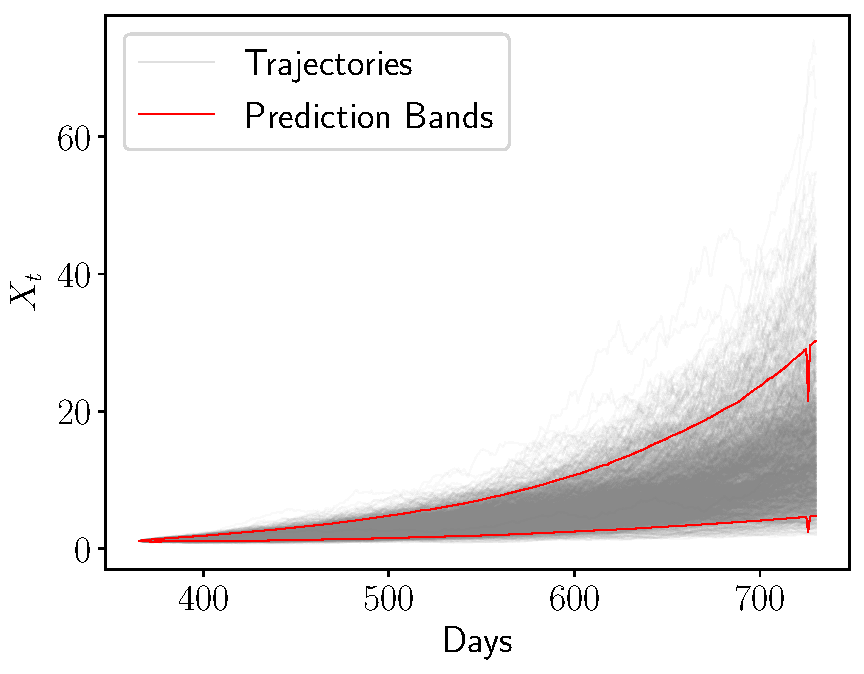
\includegraphics[scale=0.45]{bands_optimistic.pdf}
      \caption{Optimistic.}
  \end{subfigure}
  \caption{Prediction bands for each scenario.}
  \label{fig:pb1}
\end{figure}

It is clearly seen that the prediction bands enclose the majority of
trajectories; furthermore, it can be observed that these bands are not
completely smooth, for example in Figure \ref{fig:pb1} (c) the bands have a
spike near the end of the simulation time. These spikes are due to the presence
of atypical points in that particular time; it is clear that these annomalies
would be corrected when the number of trajectories considered is increased.
The percentage of effectiveness was calculated by checking how
many points longitudinally are inside the bands for each scenario. The
histogram of the effectiveness are shown Figure \ref{fig:eff1}.

\begin{figure}[H]
  \centering
  \begin{subfigure}[b]{0.45\textwidth}
      \centering
      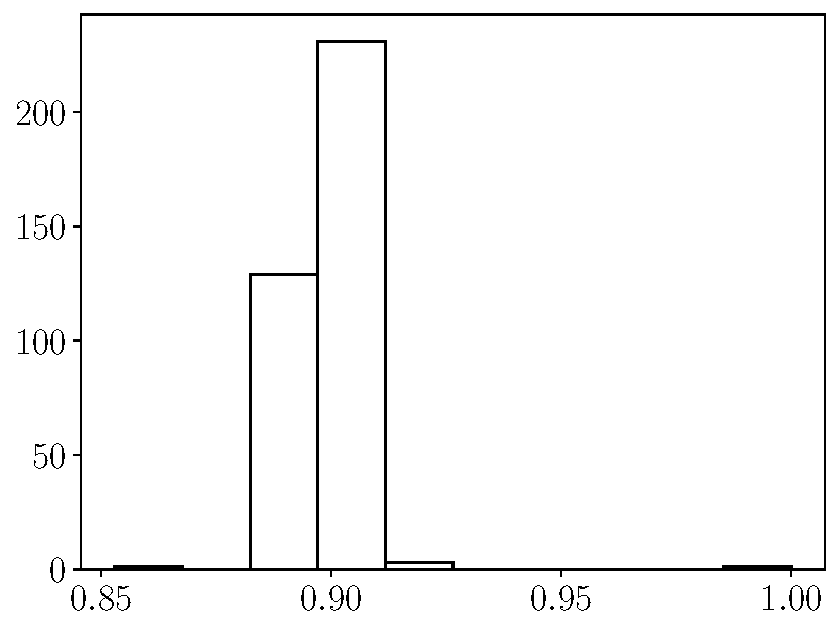
\includegraphics[scale=0.45]{eff_constant.pdf}
      \caption{Constant.}
  \end{subfigure}
  \begin{subfigure}[b]{0.45\textwidth}
      \centering
      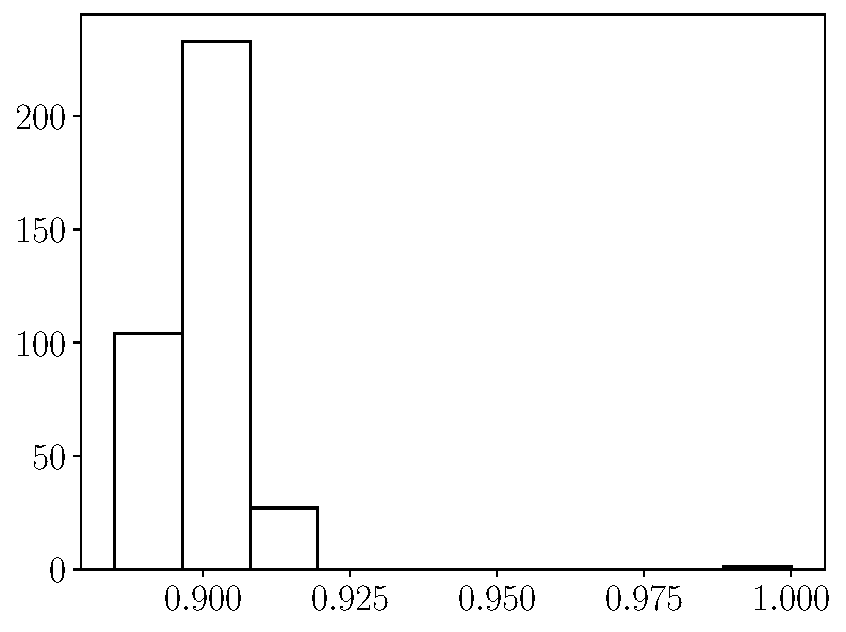
\includegraphics[scale=0.45]{eff_pess.pdf}
      \caption{Pessimistic.}
  \end{subfigure}
  \begin{subfigure}[b]{0.45\textwidth}
      \centering
      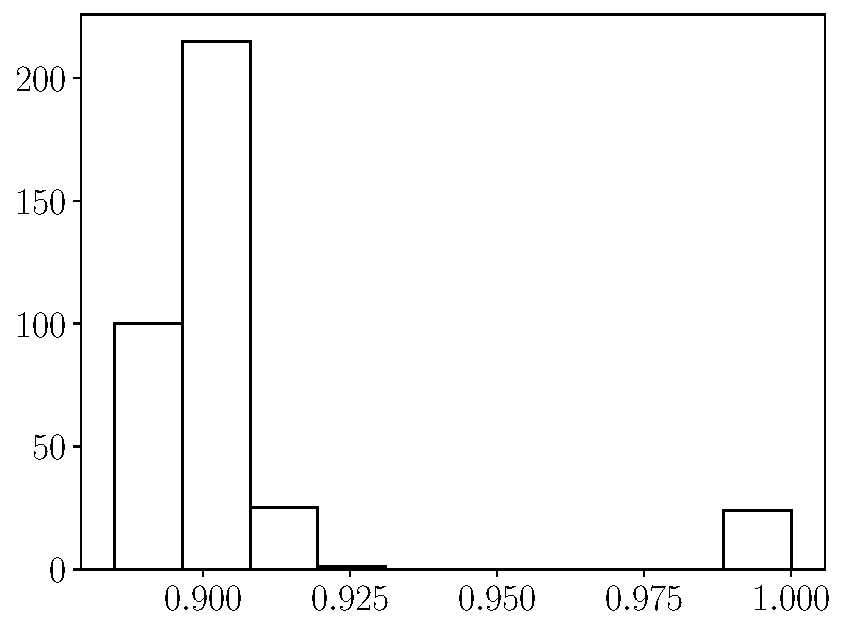
\includegraphics[scale=0.45]{eff_opti.pdf}
      \caption{Optimistic.}
  \end{subfigure}
  \caption{Effectiveness of bands for each scenario.}
  \label{fig:eff1}
\end{figure}

In conclusion, an algorithm to calculate a prediction band was
developed and successfully implemented. Furthermore, this band satisfies that
approximately $1 - \alpha$ percentage of the
trajectories are inside the bands, according to the results obtained in
\ref{fig:eff1} where the mode of enclosement is around $1 - \alpha$.

A sensitivity analysis was done for the parameter $\sigma$. The
analysis changed the respective parameter in the following manner:
\begin{equation*}
  \sigma^* = (1 + p)\sigma, \quad p \in [-0.5, 0.5]
\end{equation*}

For each value of $\sigma^*$, on each scenario, the prediction band
was calculated and the last value of the band was saved in order to summarize
the behavior of the bands when the parameter changes. In Figure
\ref{fig:sens1}, these values for each $\sigma^*$ are presented.

\begin{figure}[H]
  \centering
  \begin{subfigure}[b]{0.45\textwidth}
      \centering
      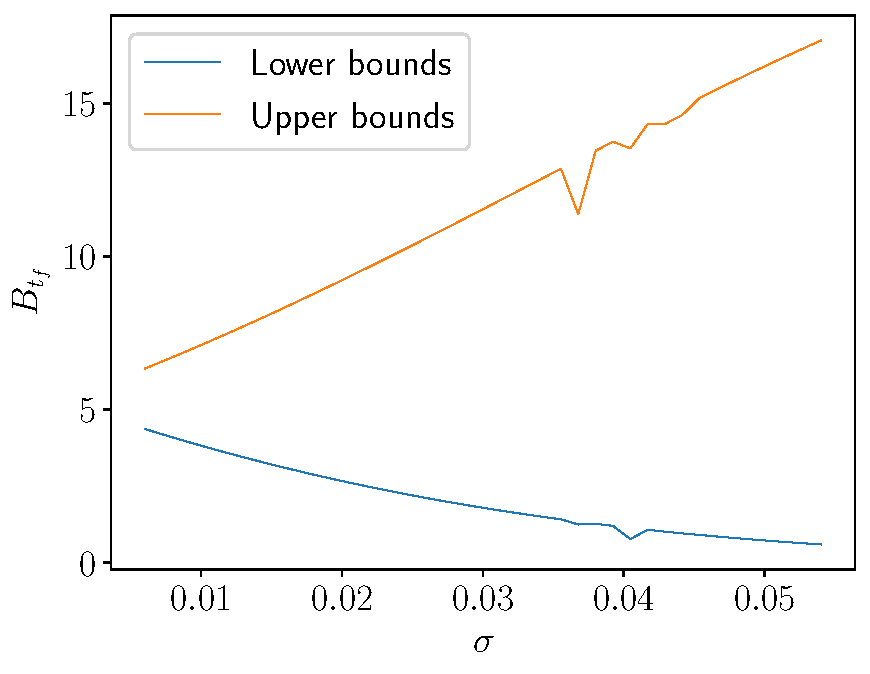
\includegraphics[scale=0.45]{sens_constant.pdf}
      \caption{Constant.}
  \end{subfigure}
  \begin{subfigure}[b]{0.45\textwidth}
      \centering
      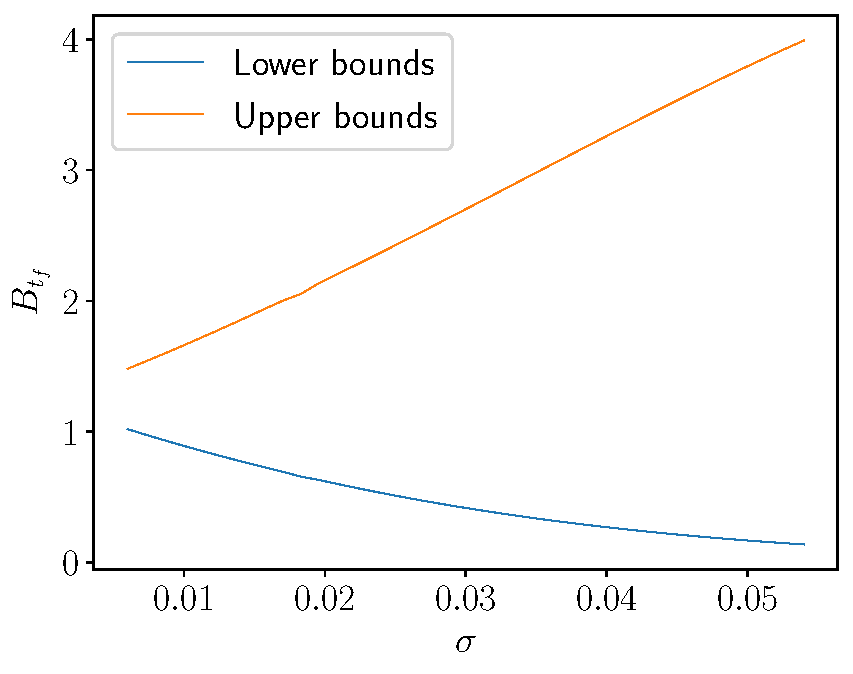
\includegraphics[scale=0.45]{sens_pessimistic.pdf}
      \caption{Pessimistic.}
  \end{subfigure}
  \begin{subfigure}[b]{0.45\textwidth}
      \centering
      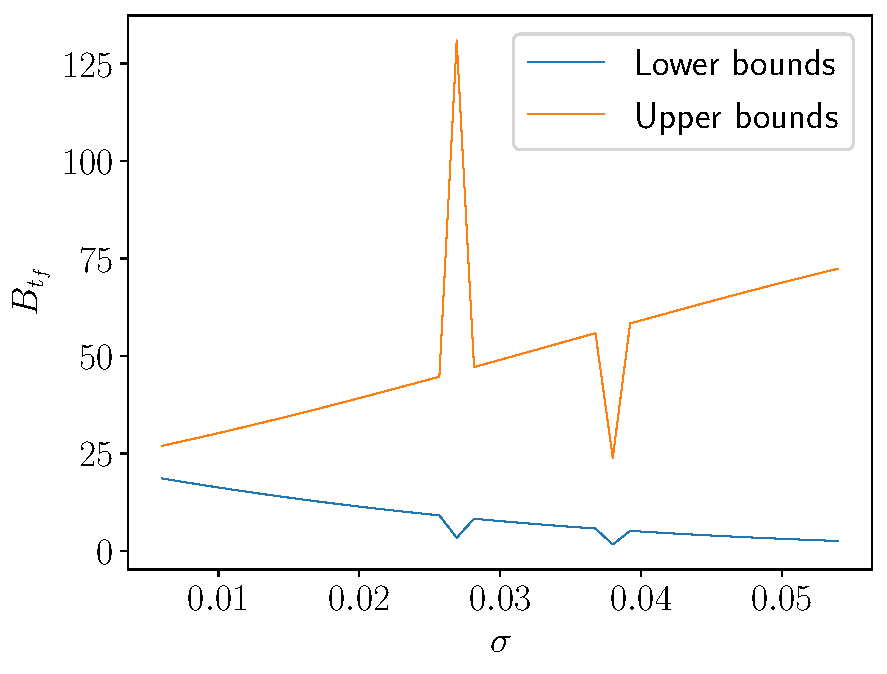
\includegraphics[scale=0.45]{sens_optimistic.pdf}
      \caption{Optimistic.}
  \end{subfigure}
  \caption{Sensitivity on $\sigma$ for each scenario.}
  \label{fig:sens1}
\end{figure}

Note that the curves for the sensitivity analysis have some annomalies, this
can be explained for the same reason why the prediction bands have spikes; the
data has unusual behavior and, again, this would be corrected if the number of
trajectories simulated is increased. Yet, the trend of these curves can still
be appreciated and it is clear that the bands get wider as $\sigma$ increases,
due to the direct relation between the volatility and the variance of the
process.

In conclusion, a sensitivity analysis on the $\sigma$ parameter was
successfully constructed and it showed the expected result: as the parameter
appears in the part related to the diffusion, augmenting it implies wider bands.

\section*{Prediction 2}
\begin{question}
  Suppose that a variable can be modeled by a Ornstein-Uhlenbeck mean
  reversion process with parameters
  $\Theta = \{\mu, \sigma, \alpha, \gamma\}$. Simulate a trajectory
  with $N = 500$ and save this trajectory (Series 2).
\end{question}

\begin{question}
  Analyze the statistical properties of Series 2. Justify the
  applicability of this equation in different knowledge areas.
\end{question}

\begin{question}
  Based on the methodology from \parencite{marin2013}, estimate the
  parameters $\{\alpha, \mu, \sigma\}$ and make an efficient forecast
  for Series 2. Establish a confidence level for the forecast and
  conclude.
\end{question}

\begin{question}
  Make a sensitivity analysis and its respective forecast for Series 2
  for parameters $\{\alpha, \mu, \sigma\}$ and conclude.
\end{question}

The mean reversion processes of one factor with constant parameters
can be written as \parencite{marin2013}:

\begin{equation*}
  dX_t = \alpha (\mu - X_t) dt + \sigma X_t^\gamma dW_t
\end{equation*}

which is also known as the Chan–Karolyi–Longstaff–Sanders process
\parencite{chan1992}, with $t_0 < t < t_f$ and
$\gamma, \sigma, \alpha, \mu \in \R_+$.

The simulation was done using the already described Euler-Maruyama scheme
with parameters: $\alpha = 2$, $\mu = 1.25$, $\sigma = 0.4$, $\gamma = 0.5$,
$\Delta t = 0.2$, $t_f = 100$, $n = 1000$. The simulation can be found in Figure
\ref{fig:series2}.

\begin{figure}[H]
  \centering
  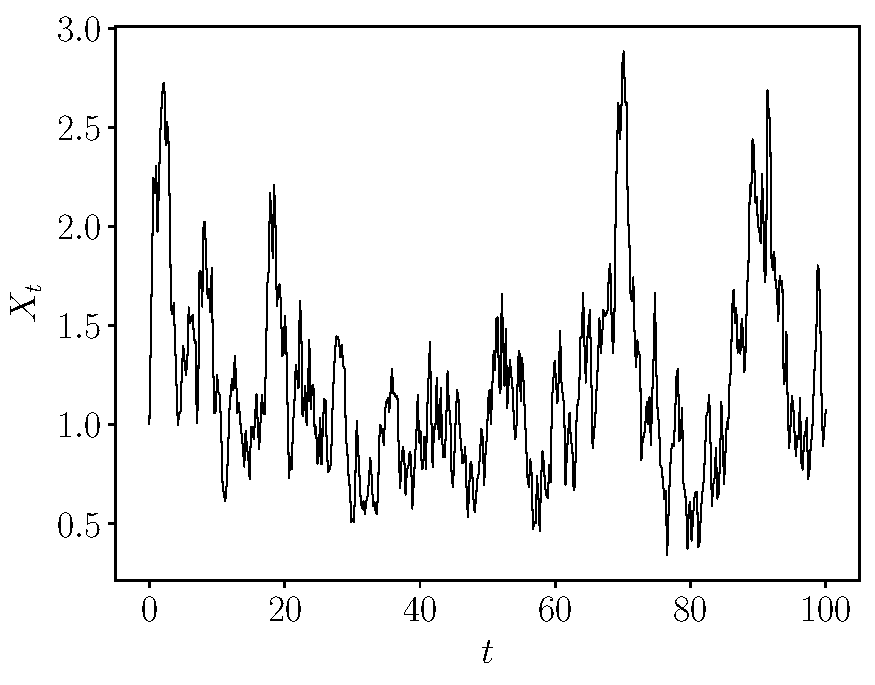
\includegraphics[scale=.5]{ornstein_serie2.pdf}
  \caption{Simulation of mean reversion process.}
  \label{fig:series2}
\end{figure}

As for the statistical properties of Series 2, the Hurst Exponent of Series 2
was calculated to check its mean reversion property, following the ideas
(and code) from \parencite{quanstart}. A time series is mean reverting if the value
of the Hurst Exponent $H$ is less than 0.5. the obtained value for this process
is $H = 0.093$.

A variance ratio test was also performed, this is a well know test for random
walks \parencite{lo1989size} and it has been widely used to test for mean
reversion (see e.g. \parencite{lo1988stock,risager1998random,lam2006new}).
The variance ratio test checks if a process is a random walk,
using the quotient of a k-period return and the return for 1 period
\parencite{charles2009variance}. Hence, a rejection of the null hypothesis
gives evidence that the process is mean reverting. The obtained result for
this test using different lags is presented in Table \ref{tab:vrt2}.

\begin{table}[H]
  \centering
  \begin{tabular}{cc}
    \hline
    lag & $p$   \\
    2   & 0.039 \\
    4   & 0     \\
    8   & 0     \\
    16  & 0     \\ \hline
  \end{tabular}
  \caption{}
  \label{tab:vrt2}
\end{table}

In this specific case where $\gamma=0.5$, the process is known as
Cox-Ingersoll-Ross (CIR) model \parencite{cox1985}. An important property
of the CIR model is that it is, almost surely, strictly positive
if $2\alpha\mu \ge \sigma^2$ \parencite{cox1985,unknown2017}, i.e.
\begin{equation*}
  \P{\text{there is at least one value of } t > 0 \text{ for which }
    X_t = 0} = 0
\end{equation*}

For further extension of the CIR model see e.g.
\parencite{overbeck1997estimation,mishra2010study,li2015asymptotic,medvedev2019cox}
This is the simplest model that allows for positive interest
rates. Furthermore, this model is useful to simulate a derivative and
future option \parencite{unknown2017}.

Another property of the CIR model is that the distribution of this process,
longitudinally, is a non-central $\chi^2$ distribution
\parencite{dyrting2004}. Although the process should follow this
distribution, in the experiments executed, only the 44\% of points in
time fitted this distribution according to a simple Kolmogorov-Smirnov test.
In Figure \ref{fig:hist_chi2} the best and worst (in a p-value sense) are presented.

\begin{figure}[H]
  \centering
  \begin{subfigure}[b]{0.45\textwidth}
    \centering
    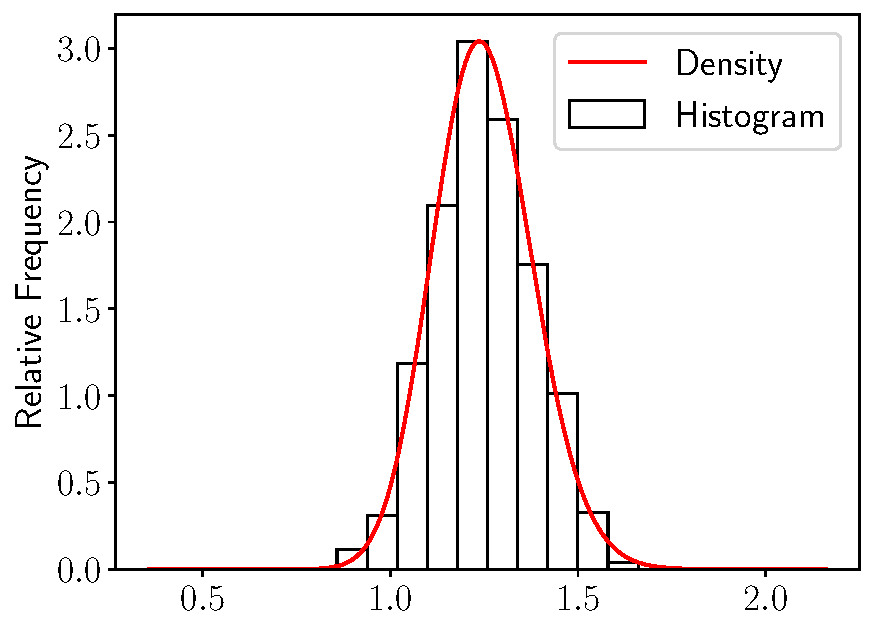
\includegraphics[scale=.45]{maxp_ncx2_histogram_eachT}
  \end{subfigure}
    \begin{subfigure}[b]{0.45\textwidth}
    \centering
    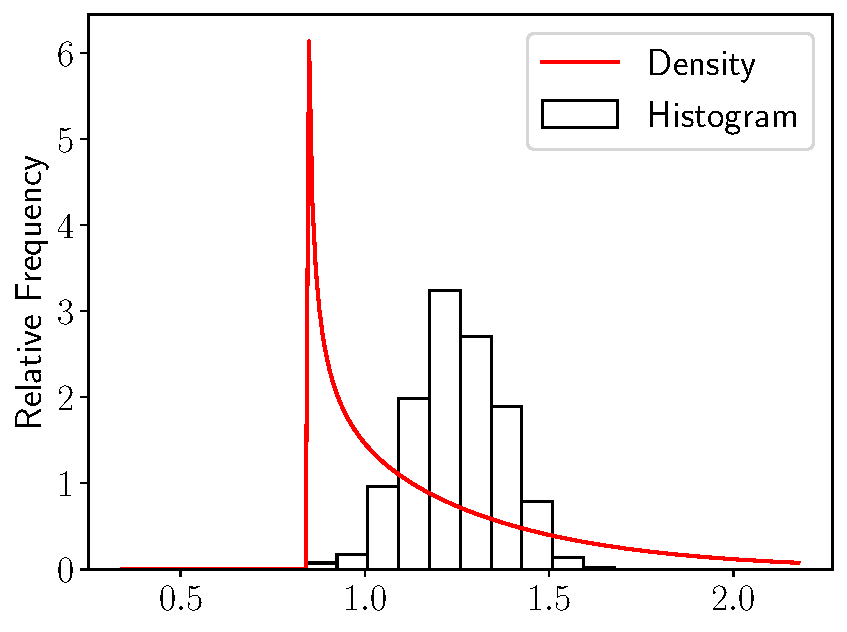
\includegraphics[scale=.45]{minp_ncx2_histogram_eachT}
  \end{subfigure}
  \caption{Best and worst non-central $\chi^2$ fitting.}
  \label{fig:hist_chi2}
\end{figure}

This may occur since $\alpha$, that is the mean reversion rate, is relatively
high, hence for the parameters chosen and for the selected time frame the CIR
process behaves similar to a white noise. Hence, by fitting a normal distribution
the 99.8\% of points in time were fitted. In Figure \ref{fig:hist_norm}
the best and worst fitting can be seen.

\begin{figure}[H]
  \centering
  \begin{subfigure}[b]{0.45\textwidth}
    \centering
    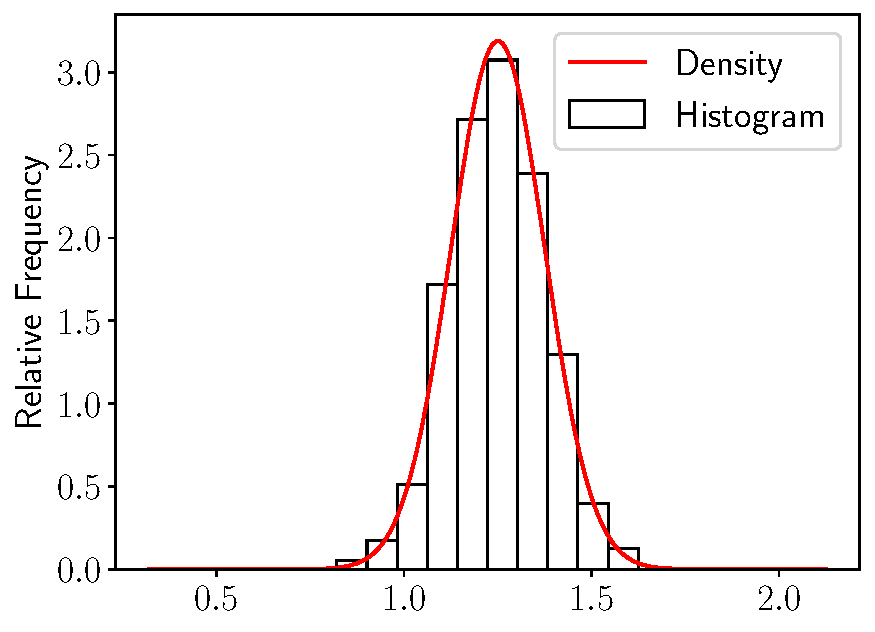
\includegraphics[scale=.45]{maxp_norm_histogram_eachT}
  \end{subfigure}
    \begin{subfigure}[b]{0.45\textwidth}
    \centering
    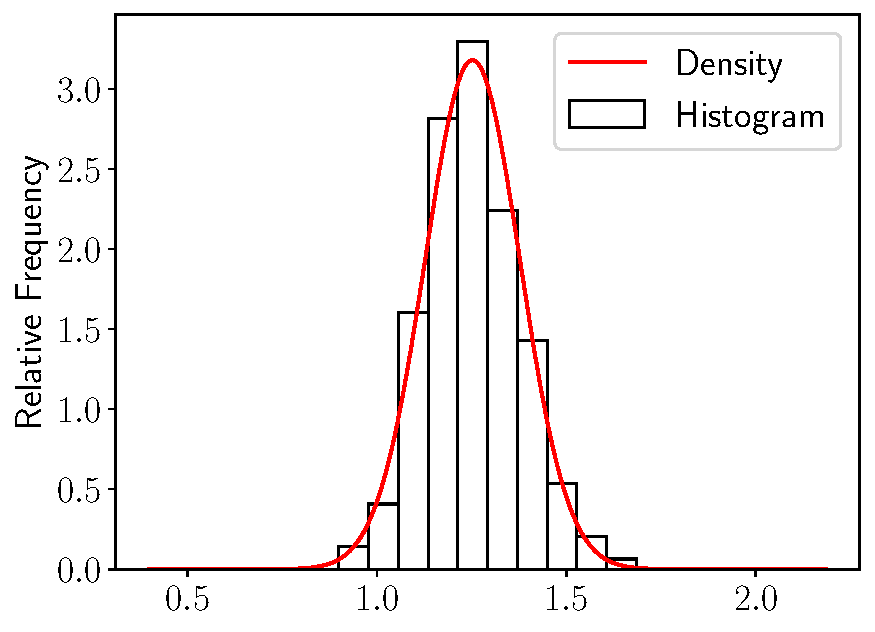
\includegraphics[scale=.45]{minp_norm_histogram_eachT}
  \end{subfigure}
  \caption{Best and worst normal fitting.}
  \label{fig:hist_norm}
\end{figure}

Furthermore, a normal distribution fitting was made transversally, which is a
string evidence of a mean-reversion-like process. The
99.7\% of trajectories were fitted. In Figure \ref{fig:hist_norm2} the
best and worst fitting can be seen.

\begin{figure}[H]
  \centering
  \begin{subfigure}[b]{0.45\textwidth}
    \centering
    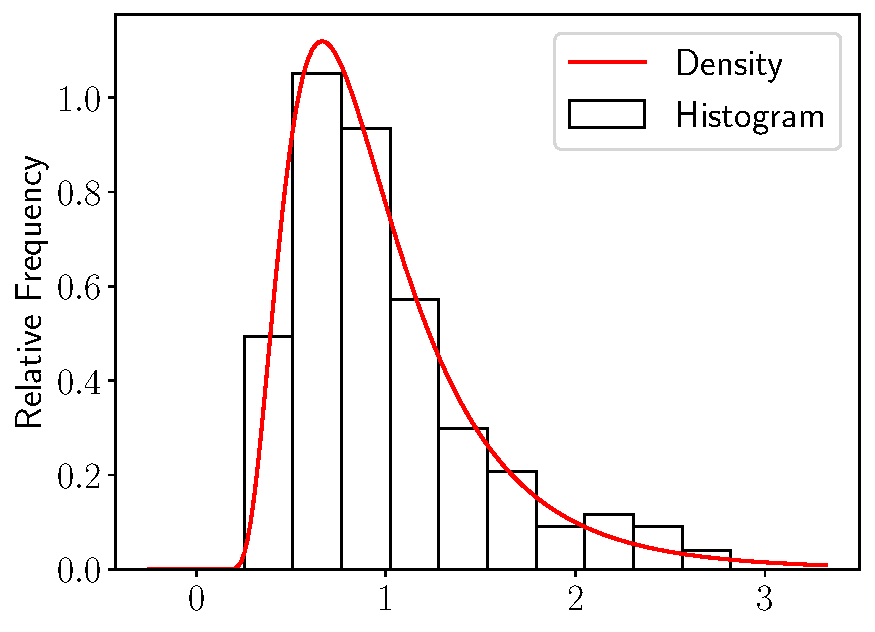
\includegraphics[scale=.45]{maxp_histogram_forallT}
  \end{subfigure}
    \begin{subfigure}[b]{0.45\textwidth}
    \centering
    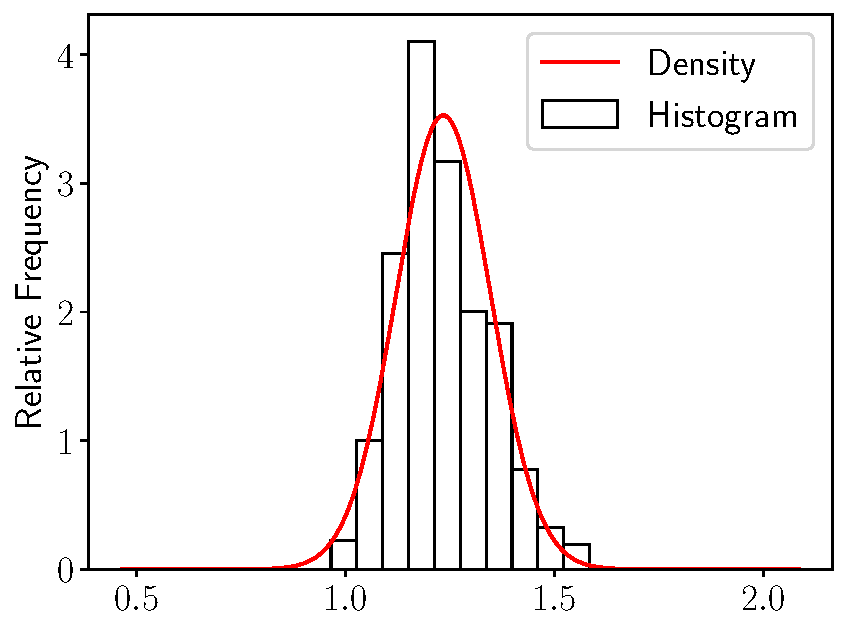
\includegraphics[scale=.45]{minp_histogram_forallT}
  \end{subfigure}
  \caption{Best and worst normal transversal fitting.}
  \label{fig:hist_norm2}
\end{figure}

The parameter estimation is done based on \cite{marin2013}.
Let $M = \left\lfloor \frac{T}{\Delta t} \right\rfloor$. The following terms
are first calculated from a sample time series:

\begin{alignat*}{2}
  &A = \sum_{i=1}^M \frac{X_iX_{i-1}}{X_{i-1}^{2\gamma}}, \quad
  B= \sum_{i=1}^M \frac{X_{i-1}}{X_{i-1}^{2\gamma}}, \quad
  &&C = \sum_{i=1}^M \frac{X_i}{X_{i-1}^{2\gamma}} \\
  &D = \sum_{i=1}^M \frac{1}{X_{i-1}^{|\gamma}}, \quad
  &&E = \sum_{i=1}^M \left(\frac{X_{i-1}}{X_{i-1}^\gamma}\right)^2
\end{alignat*}

Then, the estimation is given by:

\begin{align*}
  &\hat{\alpha} = \frac{ED - B^2 - AD + BC}{(ED - B^2)\Delta t}, \quad
    \hat{\mu} = \frac{A - E(1 - \hat{\alpha} \Delta t)}{\hat{\alpha} B \Delta t} \\
  &\hat{\sigma} = \sqrt{\frac{1}{M \Delta t} \sum_{i=1}^M
    \left(\frac{X_i - X_{i-1} - \hat{\alpha}(\hat{\mu} - X_{i-1})\Delta t}{
    X_{i-1}^\gamma}\right)^2}
\end{align*}

In order to see the behavior of this estimation, it was
done for each trajectory and the number of observations was
modified. The parameter estimation was done in different time frames
of the form $[0, \tilde{t}]$. In Figure \ref{fig:conv_param} the
average of the estimated parameters for each trajectory is seen.

\begin{figure}[H]
  \centering
  \begin{subfigure}[b]{0.45\textwidth}
      \centering
      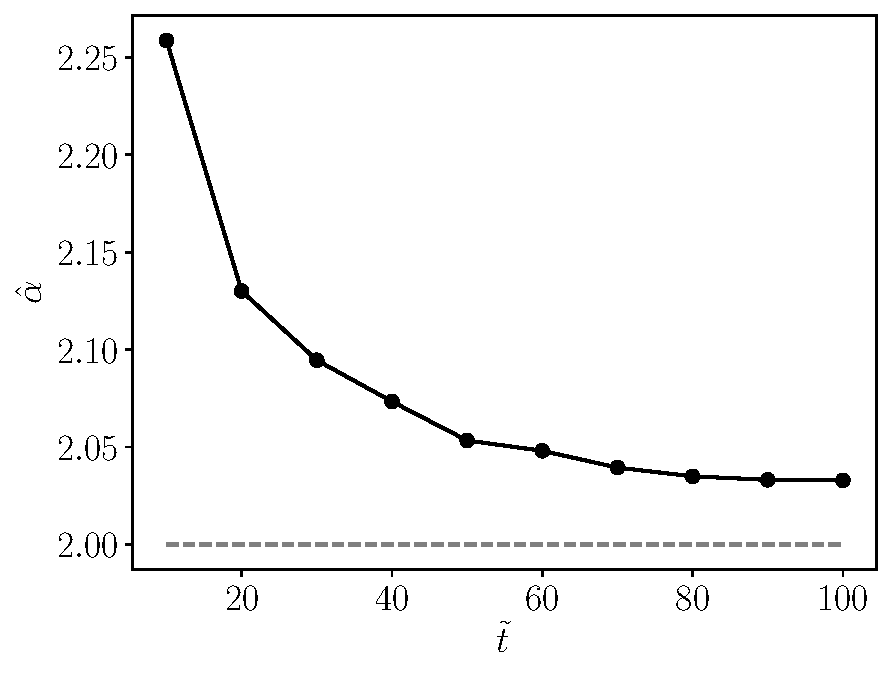
\includegraphics[scale=0.45]{alphas.pdf}
      \caption{}
  \end{subfigure}
  \begin{subfigure}[b]{0.45\textwidth}
      \centering
      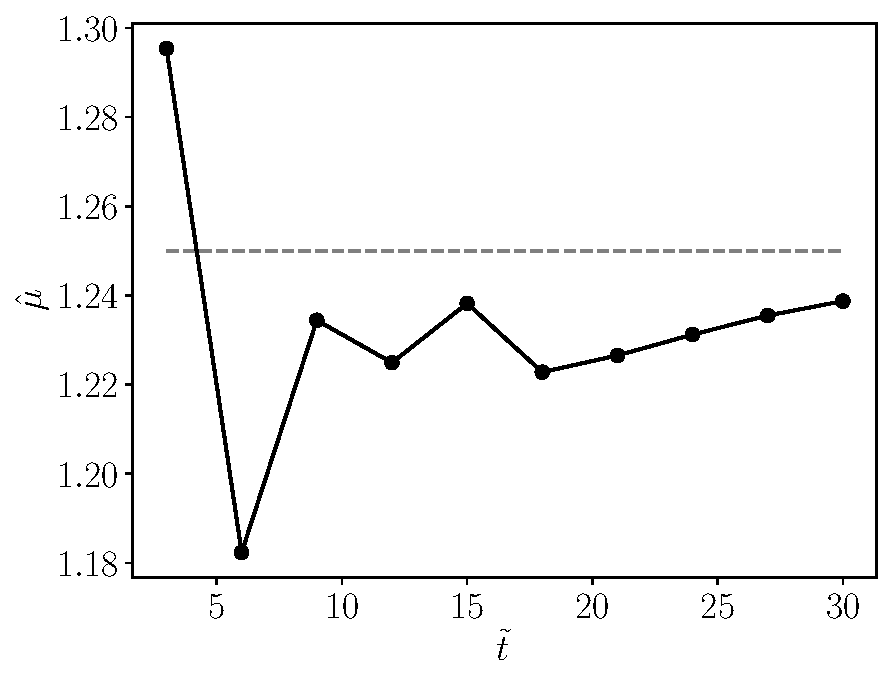
\includegraphics[scale=0.45]{mus.pdf}
      \caption{}
  \end{subfigure}
  \begin{subfigure}[b]{0.45\textwidth}
      \centering
      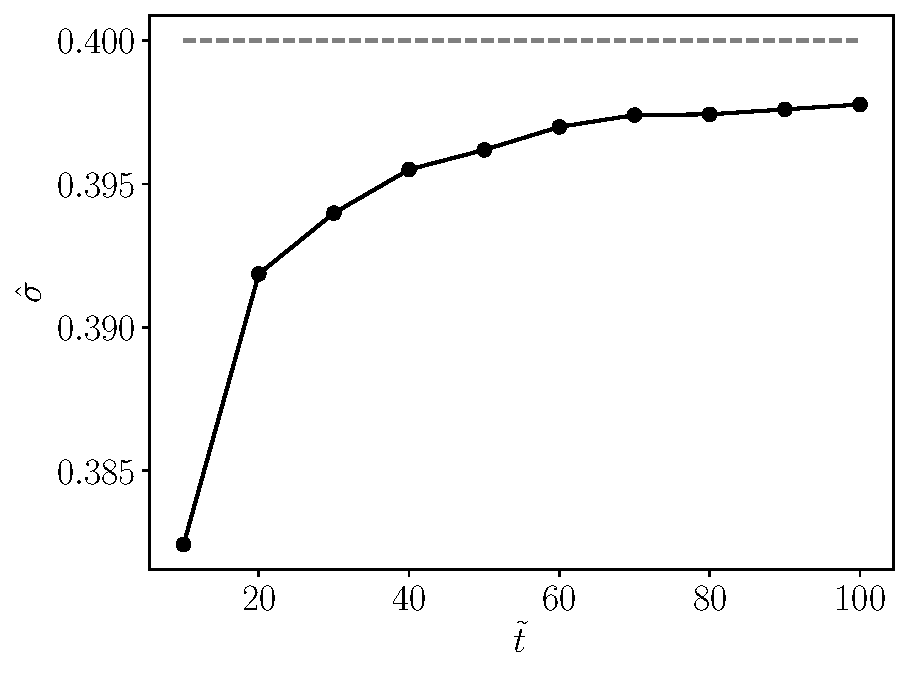
\includegraphics[scale=0.45]{sigmas.pdf}
      \caption{}
  \end{subfigure}
  \caption{Convergence of parameter estimation.}
  \label{fig:conv_param}
\end{figure}

It can be clearly observed that the parameters tend to converge on the true
values as $\tilde{t}$ increases, and consequently, the sample size increases.
Following the same procedure as the one in the previous section,
prediction bands were constructed using the fitted distributions
longitudinally. In Figure \ref{fig:bands2} the predictions bands are
displayed.

\begin{figure}[H]
  \centering
  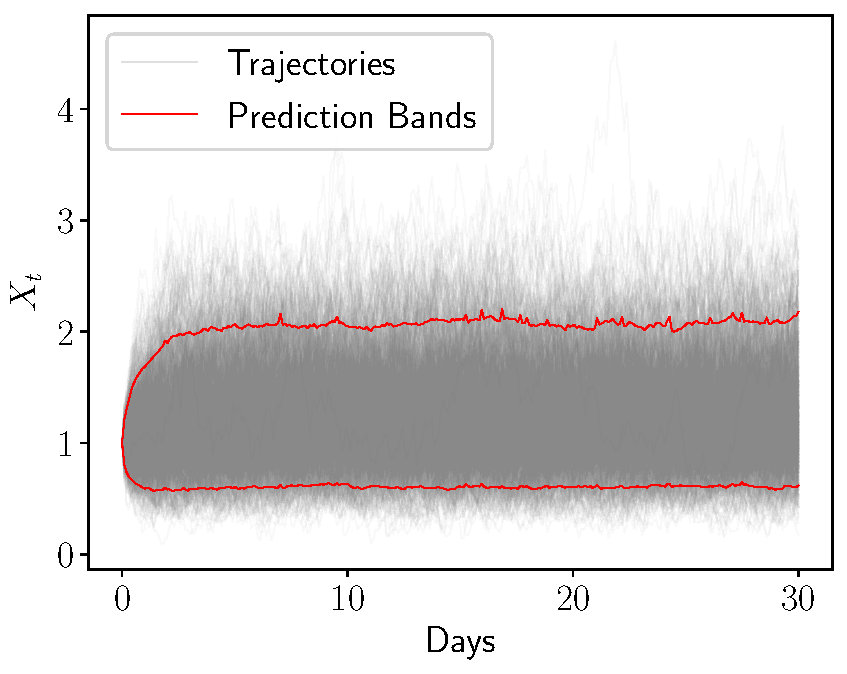
\includegraphics[scale=.5]{prediction_bands_2}
  \caption{Prediction bands for CIR model.}
  \label{fig:bands2}
\end{figure}

Finally, a sensitivity analysis was made for parameters
$\alpha, \mu, \sigma$ using the same methodology already presented in
prediction 1, but using $p \in [-0.25, 0.25]$. In Figure \ref{fig:anal2},
the sensitivity analysis for each parameter is presented.

\begin{figure}[H]
  \centering
  \begin{subfigure}[b]{0.45\textwidth}
      \centering
      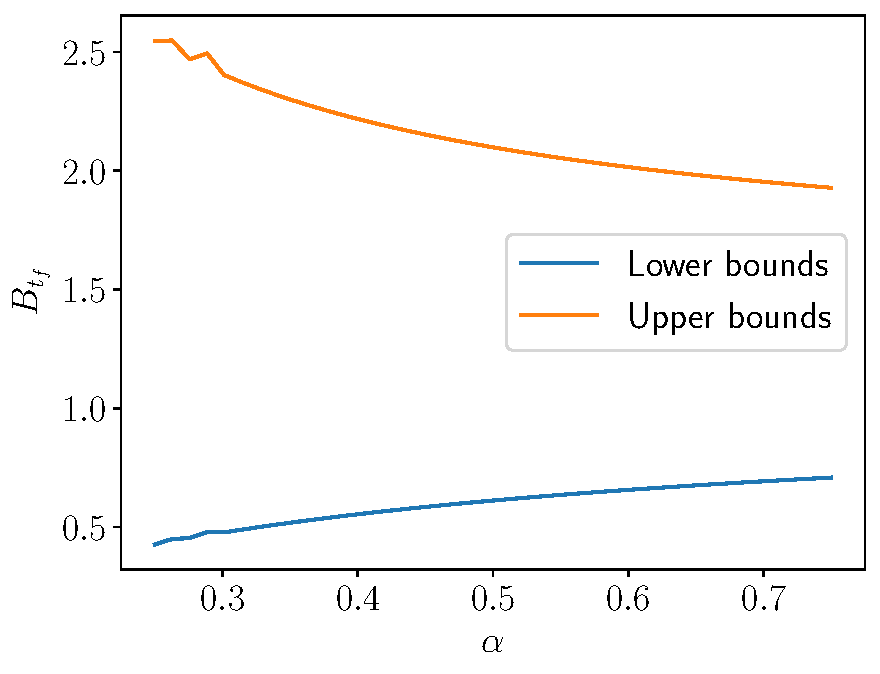
\includegraphics[scale=0.45]{alpha_sens}
      \caption{}
  \end{subfigure}
  \begin{subfigure}[b]{0.45\textwidth}
      \centering
      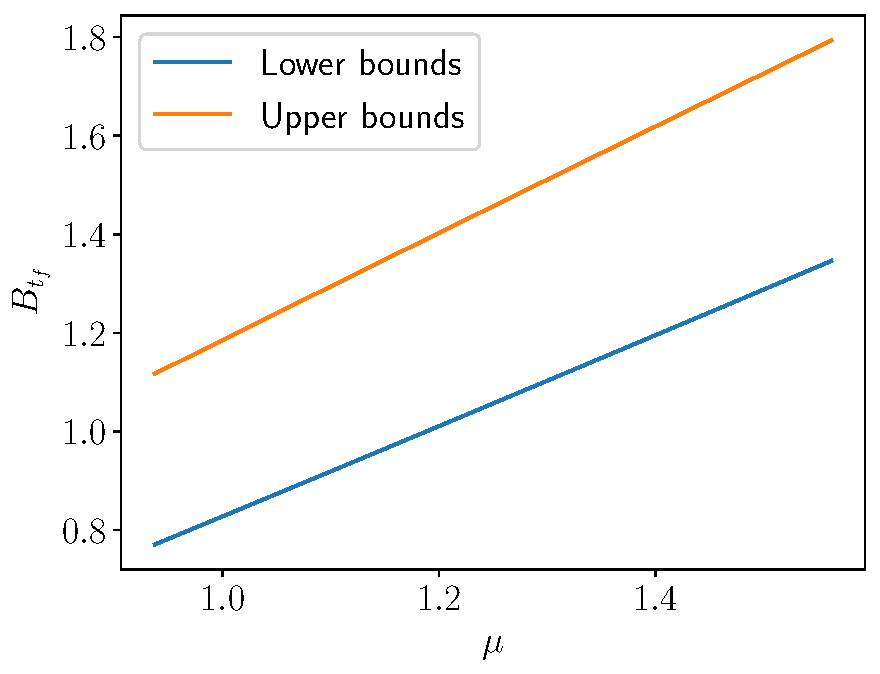
\includegraphics[scale=0.45]{mu_sens}
      \caption{}
  \end{subfigure}
  \begin{subfigure}[b]{0.45\textwidth}
      \centering
      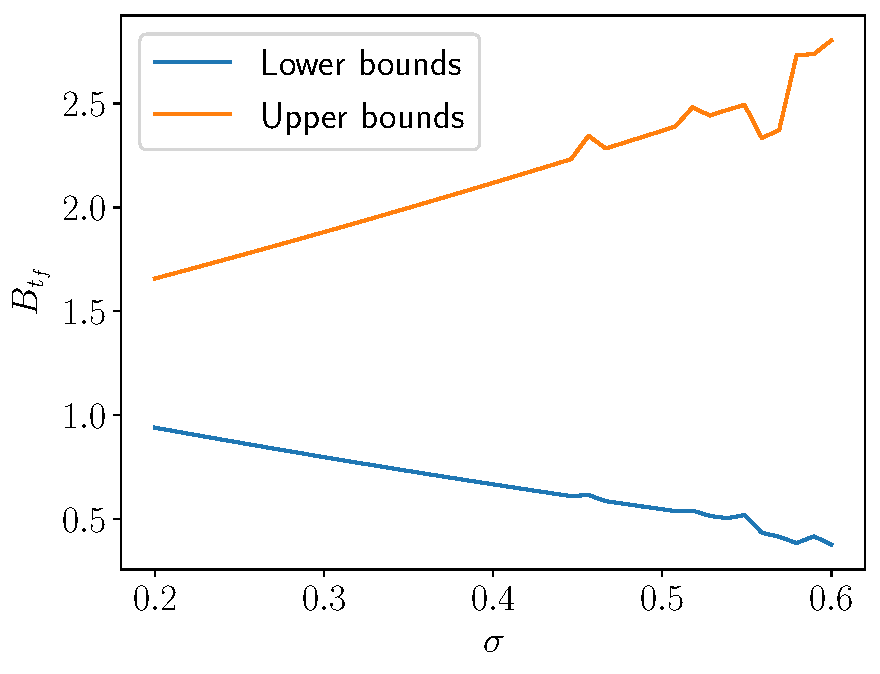
\includegraphics[scale=0.45]{sigma_sens}
      \caption{}
  \end{subfigure}
  \caption{Sensitivity analysis for parameters.}
  \label{fig:anal2}
\end{figure}

From Figure \ref{fig:anal2} (a), it can be concluded that the prediction bands
tend to get thiner as the parameter $\alpha$ increases; recall that $\alpha$
represents the mean reversion rate, therefore, if it is increased, the process
will "recover" faster implying that the trajectories will accumulate
closer to the mean and, finally, the bands capture this behavior. Additionally,
it is clear from Figure \ref{fig:anal2} (b) that $\mu$ is closely related to
the mean that the process reverts to, since an almost linear relationship
between $\mu$ and the prediction bands was obtained; the higher the $\mu$,
the higher the bands, with constant amplitude. Finally, Figure \ref{fig:anal2} (c)
shows that the bands get wider as $\sigma$ increases, and this can be justified
with a similar argument than the one in the sensitivity analysis of prediction
1: as $\sigma$ appears in the diffusion component, it has a proportional
relation with the variance of the process.

\section*{Prediction 3}
\begin{question}
  Download the data of the daily temperatures of a region of the
  northern hemisphere during at least two years. In such series a
  trigonometric periodic functional trend must be visible.
\end{question}

\begin{question}
  Analyze the statistical properties of the data and make a brief
  description of the region being analyzed.
\end{question}

\begin{question}
  Following the methodology from \parencite{alaton2002} estimate the
  parameters for a mean reversion process.
\end{question}

\begin{question}
  Make an efficient forecast for a time equal to the estimation
  period and conclude.
\end{question}

The data considered is given by Henry Laniado for another
subject. This data considers the average daily temperature in Canada
for the last 35 years. The four-most early years were extracted.
The data can be seen in Figure \ref{fig:series3}.

\begin{figure}[H]
  \centering
  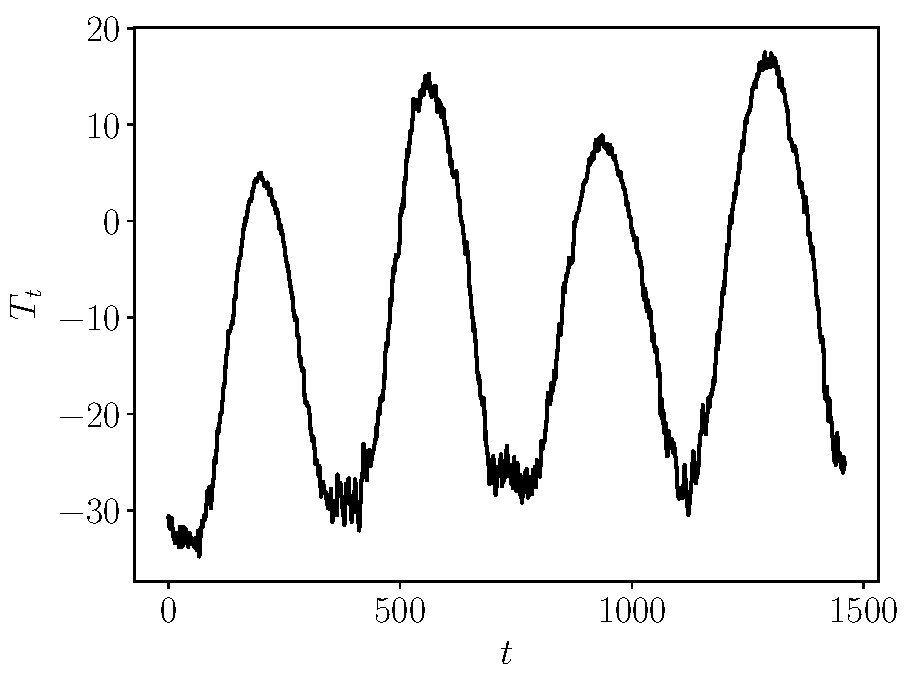
\includegraphics[scale=0.5]{temps.pdf}
  \caption{Daily temperatures.}
  \label{fig:series3}
\end{figure}

In first place, the same methodology to test mean reversion used in
last section was applied with this series. The results are presented
in Table \ref{tab:lags3}.

\begin{table}[H]
  \centering
  \begin{tabular}{cc}
    \hline
    lag & $p-value$   \\
    2   & 0 \\
    4   & 0     \\
    8   & 0     \\
    16  & 0 \\ \hline
  \end{tabular}
  \caption{Result of Variance Ratio Test.}
  \label{tab:lags3}
\end{table}

It is clear that the ratio variance test shows that the process is
mean reverting, as the null hypothesis of random-walk is rejected.

Following the ideas from \parencite{alaton2002}, it was desired to see
the behavior of the differences of adjacent daily temperatures which
can be interpreted as the Driving Noise Process. In Figure
\ref{fig:diff} it can be found the time series for the difference.

\begin{figure}[H]
  \centering
  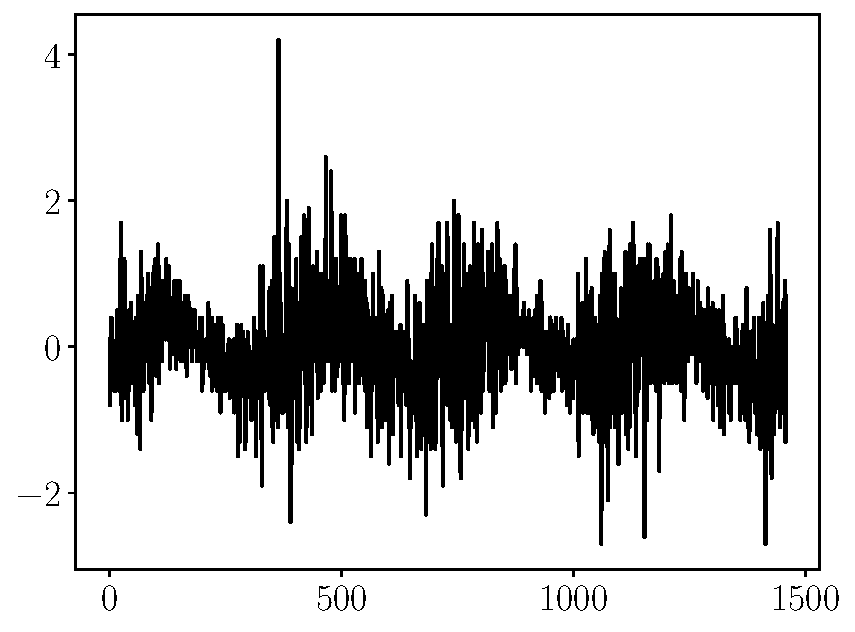
\includegraphics[scale=.5]{diffs_temps.pdf}
  \caption{Time series for the Driving Noise Process.}
  \label{fig:diff}
\end{figure}

The time series appears to be white noise with a small tendency. Hence, a normal
distribution was fitted to the time series to verify this. In Figure
\ref{fig:wn} it can be seen the fitted distribution and the histogram
of the time series.

\begin{figure}[H]
  \centering
  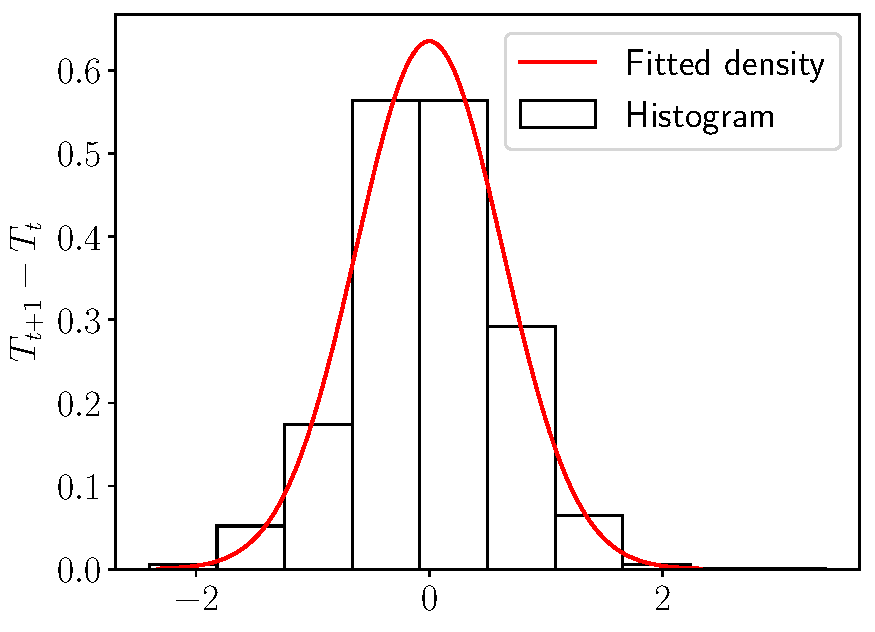
\includegraphics[scale=.5]{hist_diffs_temps.pdf}
  \caption{Fitted distrbution and histogram for Driving Noise Process.}
  \label{fig:wn}
\end{figure}

Based on \parencite{alaton2002}, the daily temperatures trend was
fitted to a process of the form:
\begin{equation*}
  T^m_t = a_1 + a_2t + a_3\sin(\omega t) + a_4\cos(\omega t)
\end{equation*}

The parameters were found using a least-squares optimization
procedure using \texttt{SciPy}. It was obtained:

\begin{equation*}
  \vv{a} = (-16.68, 9.01 \times 10^{-3}, 7.20, -18.87)
\end{equation*}

In Figure \ref{fig:trend} the adjusted trend and time series can be
seen.

\begin{figure}[H]
  \centering
  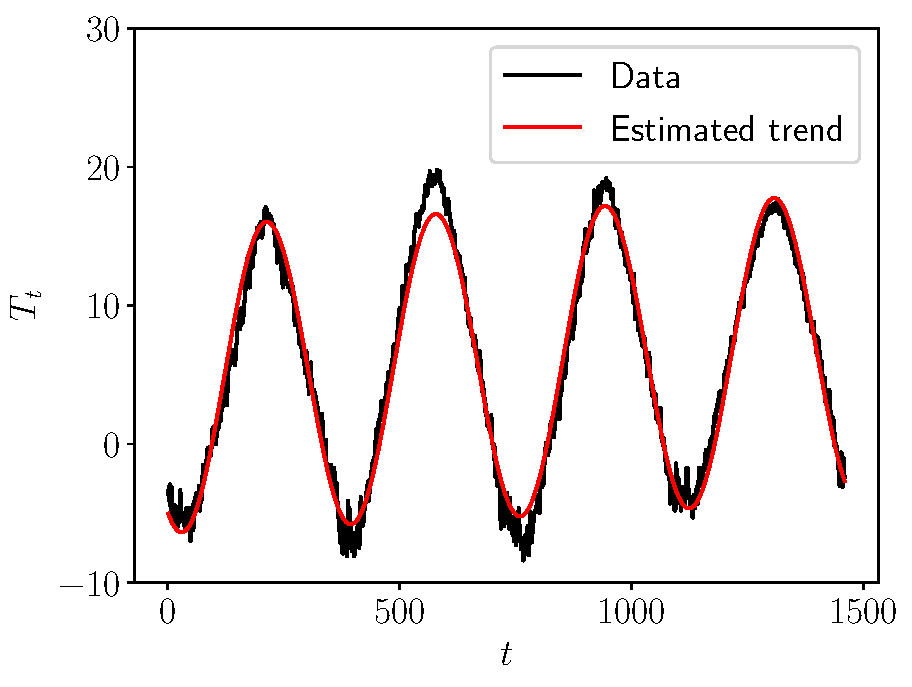
\includegraphics[scale=.5]{sine_trend.pdf}
  \caption{Trend and daily temperatures.}
  \label{fig:trend}
\end{figure}

The time series is desired to be fitted to a Ornstein-Uhlenbeck
Process, given by:

\begin{equation*}
  dT_t = \alpha(T_t^m - T_t)dt + \sigma_t dW_t
\end{equation*}

with $T_t^m$ being the adjusted trend. The procedure to estimate the
parameters is:

\begin{enumerate}
\item Let $N_\mu$ be the days in a month $\mu$ and $T_j$ be the
  temperatures in day $j$. A initial estimation for $\sigma$ in each month is
  calculated by:
  \begin{equation*}
    \hat{\sigma}_\mu^2 = \frac{1}{N_\mu}\sum_{j=0}^{N_\mu - 1} (T_{j+1} - T_j)^2
  \end{equation*}

\item Then, an estimation for $\hat{\alpha}$ is done by the following
  equation:
  \begin{equation*}
    \hat{\alpha} = \dfrac{\displaystyle\sum_{i=1}^nY_{i-1}(T_i - T_i^m)}{
      \displaystyle\sum_{i=1}^nY_{i-1} (T_{i-1} - T_{i-1}^m)}, \quad
    \text{where } Y_i = \frac{T_{i}^m - T_{i}}{\sigma_i^2}
  \end{equation*}
\end{enumerate}

In Figure \ref{fig:estimated3} the mean of 1000 simulations of the
mean reverting process and the daily temperatures can be seen.

\begin{figure}[H]
  \centering
  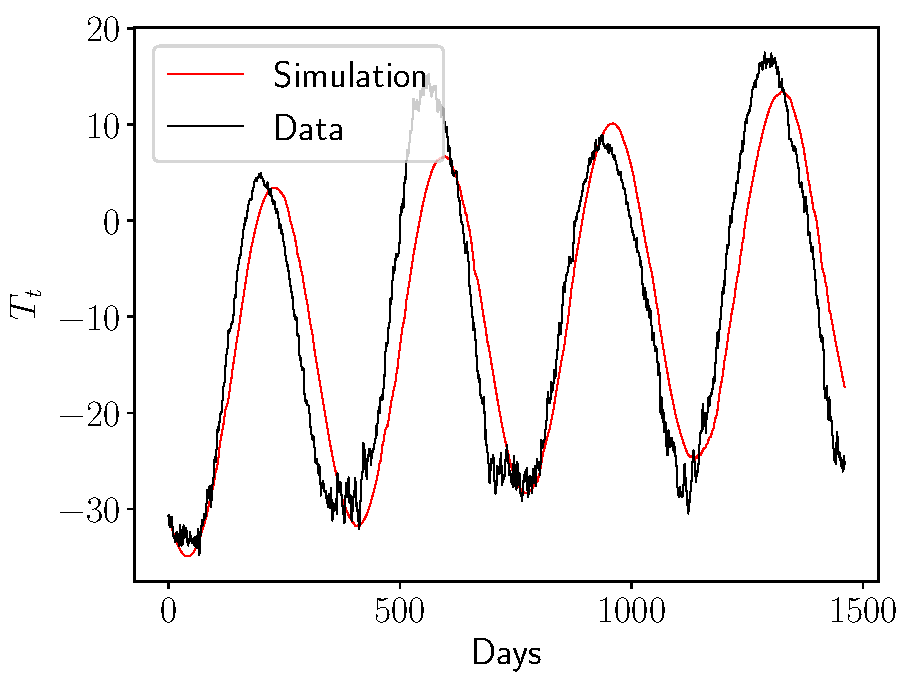
\includegraphics[scale=.5]{estimated_temps.pdf}
  \caption{Simulation and temperatures.}
  \label{fig:estimated3}
\end{figure}

Using the process with the estimated parameters, it is possible to
make a forecast of another four years. Furthermore, a comparison can be made
taking the real data of those corresponding four years and the forecast. In Figure
\ref{fig:pred3} the prediction done by the SDE and the real data are
shown.

\begin{figure}[H]
  \centering
  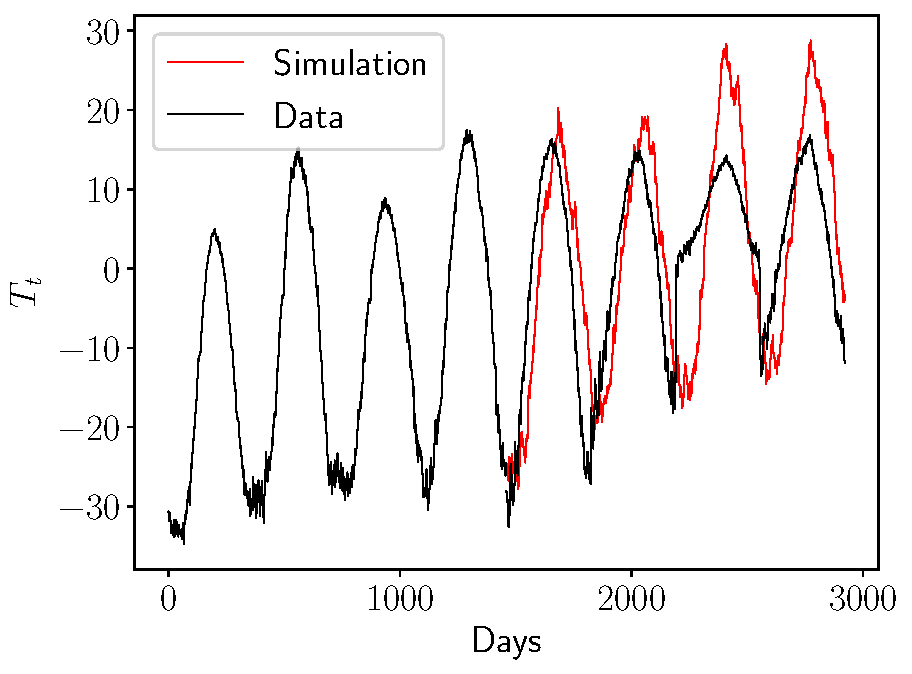
\includegraphics[scale=.5]{pred_estimated_temps.pdf}
  \caption{Mean reverting process and real data.}
  \label{fig:pred3}
\end{figure}

It is important to notice that the estimated process is a very close
approximation to the real data. In the second year forward the
approximation differs from the real data. This occurs because the data
has an unusual behavior, therefore if the real data continued its
tendency the approximation would have been much better.

It is seen that the data does not follow the linear tendency when the
predictions differs. In this manner, the authors suggest adding a term
to the tendency equation, for example adding a higher degree
polynomial.

Finally, the respective prediction bands can be constructed, using the fitted
distribution of the driving noise. Once more, 1000 trajectories were simulated
and the obtained bands (using the same procedure already described) are
presented in Figure \ref{fig:bands3}.

\begin{figure}[H]
  \centering
  \includegraphics[scale=.5]{bands_prediction3.pdf}
  \caption{Prediction bands for temperatures prediction.}
  \label{fig:bands3}
\end{figure}

\FloatBarrier
\printbibliography
\end{document}
